\documentclass[a4paper,twoside,12pt,chapterprefix=false]{scrbook}

\usepackage{amsmath,amssymb,amsthm, mathtools}
\usepackage[footnotesize,sl,SL,hang,tight]{subfigure}  % helpful package for aligning figures next to each other
\usepackage{longtable} % tables over several pages
\usepackage[font={small,sl},hang,labelfont=bf]{caption} % configure captions
\usepackage{float} % floating objects
%\usepackage{captcont} % continue sufigures over several pages
\usepackage{booktabs} % publication quality tables for LaTeX
%\usepackage{showkeys} % shows the labels above the references for easier development


\ifpdfoutput{%
	\usepackage[pdftex]{graphicx}
	\usepackage[]{pdfpages} %for including full pdf pages
}{%
	\usepackage{graphicx}
}
\usepackage{rotating} % rotate figures

\usepackage{scrpage2}
\KOMAoptions{headinclude}

% Font packages:
\usepackage{times}
\usepackage{helvet}   % sets sans serif font
\usepackage[T1]{fontenc}

%PDF hyperref config
\ifpdfoutput{%
	\usepackage[pdftex,
		bookmarks,
		bookmarksopen=true,
		bookmarksnumbered=true,
		pdfauthor={My Name},
		pdftitle={Thesis Title},
		colorlinks,
		linkcolor=black,
		citecolor=black,
		filecolor=black,
		urlcolor=black,
		anchorcolor=black,
		menucolor=black,
		breaklinks=true,
		pageanchor=true,
		plainpages=false,
		pdfpagelabels=true]{hyperref}
}{}

\ifpdfoutput{%
	\pdfcompresslevel=9
	\pdfoutput=1
	\DeclareGraphicsExtensions{.pdf,.png}
}{}

\bibliographystyle{alpha}

% Uncomment the chapter / section you are working on.
%
%\includeonly{figures}
%\includeonly{tables}
%\includeonly{data-analysis}
%\includeonly{conclusion}
%\includeonly{apx-sample-appendix}

%\pagestyle{useheadings}

% A4
%
\topmargin -0.5in
\textheight 9.3in
\textwidth 6.3in
\oddsidemargin 0.18in
\evensidemargin -0.22in
\parskip 0.1in
\parindent 0in

\renewcommand{\arraystretch}{1.5}
\renewcommand{\baselinestretch}{1}

% commands
\newcommand{\Adjoint}{\mbox{\rm Adj}}
\newcommand{\Area}{\mbox{\rm Area}}
\newcommand{\ACos}{{\mbox{\rm Cos}^{-1}}}
\newcommand{\ASin}{{\mbox{\rm Sin}^{-1}}}
\newcommand{\ATan}{{\mbox{\rm atan2}}}
\newcommand{\Code}[1]{{\tt #1}}
\newcommand{\Complex}{\mbox{\bf C}}
\newcommand{\Cross}{{\mbox{\rm Cross}}}
\newcommand{\Mydddot}[1]{\mbox{\shortstack{$.$\hspace*{-1pt}$.$\hspace*{-1pt}$.$\\$#1$}}}
\newcommand{\Degree}{\mbox{\rm degree}}
\newcommand{\Diag}{\mbox{\rm Diag}}
\newcommand{\Dim}{\mbox{\rm dim}}
\newcommand{\Dist}{\mbox{\rm Distance}}
\newcommand{\IntTwo}{\int\!\!\int}
\newcommand{\IntThree}{\int\!\!\int\! \!\int}
\newcommand{\Kernel}{\mbox{\rm kernel}}
\newcommand{\Kross}{\mbox{\rm Kross}}
\newcommand{\Grad}{\nabla}
\newcommand{\Perp}{\mbox{\rm Perp}}
\newcommand{\Point}[1]{{\cal #1}}
\newcommand{\Rank}{\mbox{\rm rank}}
\newcommand{\Range}{\mbox{\rm range}}
\newcommand{\Real}{{\mbox{\rm I}\hspace*{-2pt}\mbox{\rm R}}}
\newcommand{\RealSbt}{{\mbox{\rm\scriptsize I}\hspace*{-2pt}\mbox{\rm\scriptsize R}}}
\newcommand{\Res}{\mbox{\rm resultant}}
\newcommand{\Sbt}[1]{{\mbox{\rm\scriptsize #1}}}
\newcommand{\MySign}{\mbox{\rm Sign}}
\newcommand{\SignSBT}{\mbox{\rm\scriptsize Sign}}
\newcommand{\Skew}{\mbox{\rm Skew}}
\newcommand{\Span}{\mbox{\rm Span}}
\newcommand{\SqrDist}{\mbox{\rm Distance$^2$}}
\newcommand{\Trace}{\mbox{\rm Trace}}
\newcommand{\TRN}{{\mbox{\rm\scriptsize T}}}
\newcommand{\Vector}[1]{\mbox{\bf #1}}
\newcommand{\VectorM}[1]{\mbox{\boldmath $#1$}}
\newcommand{\Volume}{\mbox{\rm Volume}}

\newcommand{\IVec}{\mbox{\boldmath $\imath$}}
\newcommand{\JVec}{\mbox{\boldmath $\jmath$}}
\newcommand{\KVec}{\mbox{\boldmath $k$}}
\newcommand{\LVec}{\mbox{\boldmath $\ell$}}
\newcommand{\RMat}{{\cal R}}
\newcommand{\QMat}{{\cal Q}}
\newcommand{\QCMat}{\overline{\cal Q}}

\newcommand{\Lerp}{\mbox{\rm lerp}}
\newcommand{\Slerp}{\mbox{\rm slerp}}
\newcommand{\Quad}{\mbox{\rm quad}}
\newcommand{\Squad}{\mbox{\rm squad}}

\newcommand{\subsubsubsection}[1]{{\sc #1}}

\newcommand{\ODer}[2]{\frac{d #1}{d #2}}
\newcommand{\ODerT}[2]{\frac{d^2 #1}{d {#2}^2}}
\newcommand{\ODerM}[3]{\frac{d #1}{d #2 \, d #3}}
\newcommand{\PDer}[2]{\frac{\partial #1}{\partial #2}}
\newcommand{\PDerT}[2]{\frac{\partial^2 #1}{\partial {#2}^2}}
\newcommand{\PDerM}[3]{\frac{\partial^2 #1}{\partial #2 \, \partial #3}}

% mass density symbol
\newcommand{\Den}{\delta}

% environments
\newenvironment{BArray}[1]{\left\{ \begin{array}{#1}}{\end{array} \right\}}
\newenvironment{Combin}{\left( \begin{array}{c}}{\end{array} \right)}
\newenvironment{Matrix}[1]{\left[ \begin{array}{#1}}{\end{array} \right]}

% "Figure" environment
\newtheorem{localFigure}{Figure}[chapter]
\newenvironment{Figure}[1]{
  \begin{center}
  \begin{minipage}{6in}
  \par\noindent\hspace*{0pt}\hrulefill
  
  \begin{localFigure} \label{#1}
}{
  \end{localFigure}
  \par\noindent\hspace*{0pt}\hrulefill
  \end{minipage}
  \end{center}
}

% "Table" environment
\newtheorem{localTable}{Table}[chapter]
\newenvironment{Table}[1]{
  \begin{center}
  \begin{minipage}{6in}
  
  \begin{localTable} \label{#1}
}{
  \end{localTable}
  \end{minipage}
  \end{center}
}

% "CDROM" environment for source code on disk
%\newenvironment{CDROM}[1]{
%  \label{#1} 
%    \includegraphics{cdrom.png} \hspace*{0.1in}{\tt PointShop3D}. \rm
%}{
%  $\bowtie$
%}

% TO DO search symbol
\newcommand{\TODO}{\mbox{\large\bf TO DO}}
\newcommand{\REFR}{\mbox{\large\bf REFR}}

%  Terminates current page and paragraph, makes sure next page starts on
%  an odd-number, and generates a completely blank page, without page markers,
%  if necessary.
\newcommand{\clearemptydoublepage}{\newpage{\pagestyle{empty}\cleardoublepage}}

%%% Shoemake's commands
\DeclareMathOperator{\prp}{\text{\scshape perp}}
\DeclareMathOperator{\rot}{rot}
\DeclareMathOperator{\N}{N}
\providecommand{\vmag}[1]{\lVert#1\rVert}
\providecommand{\mutate}[1]{\overleftarrow{#1}}
\providecommand{\T}[1]{{#1}^{\mathrm T}}
\newcommand{\cross}{\times}
\newcommand{\by}{\times}
\newcommand{\vect}[1]{\mathbf{#1}}
\newcommand{\mat}[1]{\mathbf{#1}} % or not
%\newcommand{\quat}[1]{\mathbf{#1}}
\newcommand{\quat}[1]{\ensuremath{\mathbf{\dot{#1}}}}
\newcommand{\vV}{\vect{v}}
\newcommand{\vU}{\vect{u}}
\newcommand{\vE}{\vect{e}}
\newcommand{\vUh}{\hat{\vect{u}}}
\newcommand{\mQ}{\mat{Q}}
\newcommand{\mR}{\mat{R}}
\newcommand{\mM}{\mat{M}}
\newcommand{\mA}{\mat{A}}
\newcommand{\mB}{\mat{B}}
\newcommand{\mI}{\mat{I}}
\newcommand{\mJ}{\mat{J}}
\newcommand{\mX}{\mat{X}}
\newcommand{\mY}{\mat{Y}}
\newcommand{\mZ}{\mat{Z}}
\newcommand{\qo}{\quat{1}}
\newcommand{\qi}{\quat{i}}
\newcommand{\qj}{\quat{j}}
\newcommand{\qk}{\quat{k}}
\newcommand{\xh}{{x}}
\newcommand{\yh}{{y}}
\newcommand{\zh}{{z}}
\newcommand{\ch}{c}
\newcommand{\sh}{s}
\newcommand{\gt}{\theta}


%%
%%
%%


\begin{document}

%% Define leading chapter pages
%
%\addtokomafont{chapter}{\setlength{\parskip}{190pt}}   % SEVERE HACK to keep spacing to chapter art work
\renewcommand*{\chapterheadstartvskip}{\vspace*{215pt}}  % different hack to keep spacing to chapter artwork
%\addtokomafont{chapter}{\rmfamily}        % remove this if you prefer sans-serif section titles
%\addtokomafont{section}{\rmfamily}        % remove this if you prefer sans-serif section titles
%\addtokomafont{subsection}{\rmfamily}     % remove this if you prefer sans-serif section titles
%\addtokomafont{subsubsection}{\rmfamily}  % remove this if you prefer sans-serif section titles
%\addtokomafont{paragraph}{\rmfamily}      % replace by \sffamily if you prefer sans-serif para titles
\addtokomafont{paragraph}{\sffamily}

\def\mychpstyleintl{%
{\noindent\setlength{\tabcolsep}{0pt}\setlength{\arrayrulewidth}{2pt}%
\begin{tabular}{c}
\\[100pt]
\begin{tabular}{lr}
\begin{tabular}{p{0.6\linewidth}}
\\
\end{tabular}
&
\begin{tabular}{p{0.4\linewidth}}
\rightline{{%
\sffamily%
\fontseries{bx}%
\fontshape{n}%
\fontsize{100}{120}%choose baselineskip to be 1.2 times font size
\selectfont
\thechapter}}
\end{tabular}
\end{tabular}\\[300pt]
\end{tabular}
}}

\newpagestyle{mychapterpagestyle}{{\protect\mychpstyleintl}{\protect\mychpstyleintl}}{}
\newpagestyle{myappendixpagestyle}{{\protect\mychpstyleintl}{\protect\mychpstyleintl}}{}
%%

%% macros e.g.
\newcommand{\mfytext}[0]{my fancy text}

%refs
\newcommand{\chpref}[1]{Chapter \ref{#1}}
\newcommand{\secref}[1]{Section \ref{#1}}
%\newcommand{\equref}[1]{Equation \ref{#1}} %better use builtin \eqref{}
\newcommand{\figref}[1]{Figure \ref{#1}}
\newcommand{\tabref}[1]{Table \ref{#1}}
\newcommand{\apxref}[1]{Appendix \ref{#1}}
%%

\hypersetup{pageanchor=false} % disabling anchors for title page to avoid warning

%% Replace this by your own design of a title page
%
%\title{Thesis Title}
%\author{My Name}
%\date{September 2042}
%\maketitle
%\clearemptydoublepage
% --- selfmade version ----
\begin{titlepage}
	\topmargin 1.0cm
	\oddsidemargin 0.0cm
	\evensidemargin 0.0cm
	%\textwidth 6.5in
	\centering
	\Huge
	\vspace{3.0cm}
	\textbf{\textsf{Cross-platform Real-time Visualization and
	Editing Interface of Breast 3D meshes}} \\[2.0cm]
	\includegraphics*[width=\textwidth]{figures/placeholderTeaser} \\
	\vspace{2.0cm}
	\sffamily
	\Large
	Luca Sichi
	\\[0.8cm]
	\large
	Bachelor Thesis
	\\
	June 2023
	\\[1.3cm]
	Dr. Endri Dibra, Dr. Beren Kaul, Prof. Dr. Markus Gross
	\vfill
	\includegraphics*[width=0.3\textwidth]{figures/ETH_logo} \hfill
    % include if work done with DisneyResearch
    %\includegraphics*[width=0.3\textwidth]{figures/DRS_logo}
    %\hfill
	\includegraphics*[width=0.3\textwidth]{figures/CGL_logo}
	\vspace{3.4cm}
\end{titlepage}
\clearemptydoublepage
%%

\hypersetup{pageanchor=true}
\pagenumbering{roman}
\setcounter{page}{1}

\chapter*{Abstract}

This thesis uses computer graphics and computer vision to capture picutres of the torso, allows the user to augment the breasts, and then show the new model to compare a possible operation. The goal is to be able to use one codebase for multiple platforms, it uses the Flutter framework, which allows compilation to different platforms. In this application the main target platforms are the web and android.

\cleardoublepage
\chapter*{Zusammenfassung}

Diese Arbeit beschäftigt sich mit der Entwicklung einer neuartigen Beispielausarbeitung. Wir untersuchen die Anforderungen, die sich für eine allgemeine Vorlage ergeben, die innerhalb der \LaTeX-Textverarbeitungsumgebung verwendet werden kann. (Und so weiter und so fort\dots) Die Zusammenfassung sollte nicht länger als eine halbe Textseite sein!


%include task description here:
\cleardoublepage
%\includegraphics[viewport=3cm 0cm 20cm 27.5cm]{task_description} %better use includepdf below!
%\includepdf{task_description}
\cleardoublepage

%include acknowledgment here:
%\include{acknowledgment}

\tableofcontents
\cleardoublepage

\addcontentsline{toc}{chapter}{List of Figures}
\listoffigures
\cleardoublepage

\addcontentsline{toc}{chapter}{List of Tables}
\listoftables
\cleardoublepage

\pagenumbering{arabic}
\renewcommand*{\chapterpagestyle}{mychapterpagestyle}
\renewcommand*{\chapterformat}{} % show chapter titles only (no numbers)
% \setchapterpreamble[o]{...}  unfortunately does not move the \chapter output downwards

% ---- MAIN PART ----

% set counter to n-1:
\setcounter{chapter}{0}

\chapter{Introduction}

\section{Background}

The main goal of this thesis is to develop a cross-platform application that allows users to modify the appearance of the breasts and evaluate the potential outcomes of a surgical procedure. 
The application is intended to be used by plastic surgeons and their patients. 

One of the primary objectives is to incorporate similar functionalities as the \textbf{Lind App}, created by Arbrea Labs, into the application. 
The aim is to establish a unified codebase capable of operating on various platforms, with a particular focus on the web and Android.



\section{Problem Statement}


% set counter to n-1:
\setcounter{chapter}{1}

\chapter{Related Work}

Sample references are~\cite{Zwicker04Perspective} and~\cite{Altman89QuaternionScandal}.

\section{Displaying 3D Models}

A pivotal aspect of this thesis revolves around the presentation of 3D models. Given the intended deployment of the application across diverse platforms, the implementation necessitates a cross-platform approach. 
To address this requirement, we derive inspiration from webGL and openGL, adapting their principles to develop a custom solution. 
Notably, a substantial portion of the rendering process is executed through the utilization of the Cube Flutter plugin, which we have tailored to align with our specific needs.


\section{Modification of 3D Models}

To facilitate the alteration of the 3D models, an adapted approach is employed, drawing inspiration from the methodology presented in the scholarly work by \textbf{Zwicker et al. (2004) titled "Perspective Shape from Shading."}

Wavefront OBJ files serve as the file format for storing the 3D models employed in this study. To facilitate their integration with the rendering engine, a parsing mechanism is implemented to extract the necessary geometric and texture information from the OBJ files. 
Subsequently, a conversion process is executed to transform the extracted data into a compatible format that can be seamlessly rendered by the rendering engine.


\chapter{Methods}

This chapter provides a detailed description of our approach, outlining the sequential steps we undertook to accomplish our goals. We present a thorough analysis of the challenges we encountered during 
the development process and offer comprehensive explanations for the decisions made in our approach.

We begin by explaining the rationale behind our chosen methodology and highlight the specific objectives we aimed to achieve. We then proceed to discuss the individual steps involved in our approach, 
providing a comprehensive overview of each stage's purpose and significance.

Throughout this chapter, we delve into the problems we encountered during the implementation of our approach. We discuss the reasoning behind the strategies adopted to address these challenges, 
providing insights into the decision-making process.

\section{Image Acquisition}

The initial phase involves the acquisition of patient data. For our specific objectives, a triad of torso images is essential, comprising a frontal view, a left lateral view, and a right lateral view. 
These images provide comprehensive visual information required for subsequent analysis and augmentation processes. Given our objective of maximizing the versatility of our application, 
we aim to enable the utilization of images from diverse sources. This entails providing users with the flexibility to capture patient images using the device's camera or select existing images from the gallery. 
By incorporating such functionality, our application caters to varying user preferences and facilitates seamless integration with different image acquisition methods, 
enhancing the overall usability and accessibility of the app.

Within the Flutter framework, a comprehensive range of image acquisition widgets is available, including the ImagePicker and Camera widgets. 
The ImagePicker widget empowers users to select an image from the gallery of the device, while the Camera widget facilitates real-time image capture utilizing the device's integrated camera 
or an external camera like a webcam. These widgets serve as essential components within the Flutter ecosystem, offering intuitive and efficient means of acquiring images from distinct sources, 
thus enhancing the flexibility and functionality of our application.

At this stage, we confront a challenge pertaining to platform-specific code. The web application, being browser-based, presents a hurdle in terms of accessing the device's memory, 
which poses inherent difficulties. In contrast, the Android platform offers seamless access to the device's memory without encountering similar obstacles. 
This distinction underscores the need for devising a solution that accommodates the limitations imposed by web-based environments, ensuring compatibility and functionality across platforms.

\subsection{Image Acquisition on Android}

Since the Android platform offers direct access to the device's memory, the implementation of the image acquisition process is relatively straightforward. 
Utilizing the Camera widget, we facilitate real-time image capture, subsequently storing the captured images within the device's memory. 

Given the requirements of Arbrea's established pipeline, 
which necessitates three torso images encompassing a frontal view, a right-side view, and a left-side view, the user is instructed to capture and retain three distinct pictures. 
We then save these images on the divece's memory and subsequently pass them to the next stage of the pipeline.

\subsection{Image Acquisition on Web}

On the web platform, our implementation deviates slightly from the Android counterpart due to the stringent restrictions on accessing the device's memory. 
To circumvent these limitations, we rely on methods inherent to web development practices. Specifically, images captured using the camera are stored within the browser environment as Binary Large Objects (BLOBs). 
This storage mechanism allows for efficient management and retrieval of image data, enabling seamless processing and integration within the web-based application.

A Blob represents a file-like object of immutable, raw data. Blobs represent data that isn't necessarily in a JavaScript-native format. 

In our web-based implementation, the Camera widget generates Binary Large Objects (BLOBs) automatically for the captured images, providing us with URLs instead of conventional file paths for subsequent referencing. 
Similar to the Android implementation, we guide the user to capture three torso images. Given that a device may possess multiple cameras or webcams, we incorporate functionality that enables the user 
to select their preferred camera. The Flutter framework proves invaluable in this regard, as it streamlines the management of diverse camera and webcam options available on the device, 
ensuring seamless compatibility and optimal utilization.

In addition to capturing images through the device's camera, we offer users the alternative option of selecting images from their device's gallery. This feature proves particularly useful 
for users operating desktop computers, where capturing satisfactory images with a webcam can be challenging and inconvenient. Given the recurring constraint of limited access to the device's memory, 
we rely on the Flutter framework to present a viable solution. Leveraging the ImagePicker widget within Flutter, users can seamlessly select or drag and drop images from their devices 
and upload them to the web application. This functionality parallels the familiar concept of file uploads on websites, a ubiquitous feature found across numerous online platforms. 
\textbf{TODO: Add image of ImagePicker widget and drag and drop}

\section{Communication with the backend Pipeline}

At this juncture, we find ourselves faced with the task of obtaining a 3D model from the captured torso images of the patient. To accomplish this, we adopt the existing pipeline developed by Arbrea Labs, 
which serves as the foundation for generating the requisite 3D model. However, to initiate this process, establishing a connection to a dedicated server hosting the pipeline becomes imperative. 
Subsequently, the client transmits the acquired images alongside additional pertinent data to the server. The server, in turn, employs the received data to invoke the pipeline, 
initiating the creation of the 3D model. Once generated, the resulting model is transmitted back to the client, where it is stored for subsequent stages of processing, augmentation, and visualization.

In light of the straightforward requirements for the server component, we have opted to utilize a basic Python server that leverages Python's built-in http.server implementation. 
This minimalistic server implementation provides the necessary functionality to handle HTTP requests and responses without the need for complex external dependencies.

\subsection{Python}

Within the server-side architecture of our application, the primary objective is to receive three images from the client. Furthermore, considering the pipeline's reliance on the distance 
between the patient's nipples, we require the client to transmit this essential information alongside a unique identifier. When a POST request is received, the server anticipates a JSON object 
comprising the three images, with the frontal image listed first, followed by the right-side image, and concluding with the left-side image. The JSON object also encompasses the distance 
between the nipples and the unique identifier.

Subsequently, the server proceeds to create a dedicated directory named after the unique identifier, serving as a repository for storing the received images. Given that the incoming 
images are not in a standard image file format, a conversion process becomes necessary. To accomplish this, we employ the Python Imaging Library (PIL), a powerful image processing library. 
By leveraging the functionalities offered by PIL, we can effectively convert the received image data into a compatible image file format that can be readily utilized within the pipeline. 

Additionally, a text file is generated within this directory, containing the recorded distance between the nipples. 
This organization ensures efficient and easy to understand data management and facilitates seamless integration within the subsequent stages of processing.

Upon completion of the image processing pipeline developed by Arbrea, the resulting 3D model is saved within the same directory as the original images. 
Our application employs the widely used Wavefront OBJ file format for storing the 3D model, utilizing three distinct files. The primary file, 
denoted with the .obj extension, contains the actual geometric data of the 3D model. Additionally, the .mtl file is employed to store material-related information, 
while the .png file serves as a repository for texture information. These three files constitute the output generated by the pipeline.

Given that both the .obj and .mtl files are text-based, they can be easily processed by reading and transmitting them as strings to the client. 
However, the texture file, being an image file, necessitates encoding prior to transmission over the HTTP connection. Within our implementation, 
we have incorporated the functionality to perform individual GET requests to the server for each file separately. This enables the 
precise retrieval of the required files from the server in a granular manner. 

\subsection{Flutter}

On the client-side of the application, an initial step involves initiating a POST request to the server. To facilitate this communication process, 
we employ the Dio package, a robust HTTP client specifically designed for Dart programming. This package provides comprehensive functionalities for 
handling HTTP requests and responses efficiently and effectively.

As previously mentioned, the server expects a JSON object as part of the POST request, comprising the three torso images in the following order: 
frontal, right-side, and left-side images. Additionally, the JSON object should include the distance between the patient's nipples and a unique identifier. 
Before transmitting the images to the server, it is necessary to encode them appropriately. To achieve this, we utilize another package, 
specifically the http package, which offers a convenient means of encoding images using the local URL of the Binary Large Object (BLOB).

It is worth noting that in scenarios where the image is uploaded or when operating within the Android environment, 
direct access to the encoded image data is available, thus bypassing the need for additional encoding steps. Following this, 
the application prompts the user to input the distance between the patient's nipples, subsequently generating a unique identifier. Finally, 
utilizing the Dio package, the POST request is dispatched to the server, facilitating the seamless transmission of the required data.

To obtain the 3D model from the server, we employ a GET request, utilizing the Dio package once again to manage the communication process. 
Our application necessitates two versions of the 3D model: one that allows modifications and augmentations to the breast area and another 
that remains unaltered. Consequently, we perform two separate GET requests to retrieve these models.

As our visualization method is based on the Flutter Package Cube, we require three GET requests per model: one for the .obj file, one for 
the .mtl file, and one for the .png file. To accommodate this requirement, we have made adaptations to the existing Cube parser to accept 
a URL instead of a local file path. The parser is then responsible for performing a GET request for each file from the server and subsequently parsing the received data.

It is important to note that Dart employs base 16 encoding for strings, unlike Python's base 64 encoding. Consequently, when working with raw data, 
particularly when performing a GET request for the .png file, caution must be exercised. We must first decode and re-encode the data appropriately 
before utilizing it within the Cube parser. This ensures compatibility and proper handling of the data within the application.

\section{Visualization of the 3D Model}

As previously discussed, the visualization of the 3D model is primarily facilitated by the integration of the Flutter package Cube. 
This package encompasses a 3D model viewer, which incorporates a standardized implementation of a computer graphics pipeline. 
In order to effectively render the 3D models, Cube relies on an internal representation of these models, which is described and structured by the object.dart file.
Understanding this representation is crucial for our application, because we want to be able to change vertices of the model, and as discussed above,
we have a different method of initializing the model.

It is worth mentioning that in cases where we have two objects within the scene, one loaded from local memory and the other fetched from the server, 
there may be a noticeable distinction in their appearance, manifesting as a bluish hue. This discrepancy arises due to the contrasting color descriptions utilized, 
specifically a mixture of RGB (Red, Green, Blue) and RGBA (Red, Green, Blue, Alpha) color formats. While this discrepancy surfaced unexpectedly during 
the debugging phase, it is essential to note that it does not significantly impact our application since we rely on the server as the source of our models.

\textbf{TODO: Add image of the two models}

In our implementation we have two screens, which display the 3D models. In the first screen we display the 3D model for breast modification. We implement three different views,
one from the front, where the model can rotate around the y-axis:

\textbf{TODO: Add image of the model from the front}

One from the top, where the model can slightly rotate around the x-axis:

\textbf{TODO: Add images from top}

And finally a view from below, in which the user can also slightly rotate the model around the x-axis:

\textbf{TODO: add images from below}

The second screen displays the modified model next to the unmodified model, where the user can compare the two models.

\textbf{TODO: Add images of the two models}

Within the object.dart file, one can locate the presence of a mesh object, as explicitly defined in the mesh.dart file. This particular mesh object encapsulates an 
array of vertices, polygons, normals, and various other essential details pertaining to the model, which collectively contribute to its visual representation. 
It is worth noting a significant but nuanced aspect, where a function is employed to duplicate vertices that possess multiple texture coordinates. 
This duplication process ensures that each vertex within the mesh object maintains a singular texture coordinate. This particular detail warrants 
consideration when attempting to manipulate the vertices of the model at a later stage.

The Cube package furnishes us with the essential transformation matrices, specifically the model, view, and projection matrices. 
These matrices are of utmost importance as they enable us to perform various transformations on the 3D model and facilitate its visualization. 
The presence of these matrices within the scene.dart file streamlines our subsequent tasks, as we can readily access and utilize them when required.

\section{Modification of the 3D Model through PCA}\label{sec:modification}

Our primary objective revolves around the ability to manipulate the 3D breast model to simulate the outcomes of a breast augmentation surgery. 
Numerous options exist to achieve this goal. However, our chosen approach entails employing the Principal Component Analysis (PCA) method, 
a statistical procedure that facilitates a substantial reduction in the dimensionality of our data. This methodology aligns with the techniques employed by Arbrea, 
thereby enabling potential future enhancements to be implemented in a manner consistent with those utilized in the Lind App.

\subsection{Principal Component Analysis}

Principal Component Analysis (PCA) is a statistical technique used to analyze and reduce the dimensionality of a dataset while preserving its essential characteristics. 
It identifies the principal components, which are linear combinations of the original variables that capture the maximum amount of variance in the data. 
By projecting the data onto these principal components, PCA enables us to interpret complex datasets like for example 3D models of the female torso. PCA aids in uncovering patterns, 
relationships, and underlying structures in high-dimensional data, making it a valuable tool for dimensionality reduction and data compression.

Due to the convenience and functionality provided by Python for performing Principal Component Analysis (PCA), we opted to conduct the PCA fitting and initial analysis in Python. 
Python offers comprehensive libraries and tools, such as scikit-learn, that facilitate the implementation of PCA and provide extensive support for data analysis and manipulation. 
By leveraging Python's capabilities, we can efficiently extract the principal components from our dataset and explore their significance and contribution to the variance. 
Subsequently, we can utilize the obtained PCA results in our Flutter application for further processing and visualization of the modified 3D models.

Our initial step involved acquiring a dataset from Arbrea, which consisted of 266 3D models. Since our objective was to modify only the vertices of the 3D models, we extracted the 
vertex information exclusively from the dataset. This resulted in a modified dataset comprising 266 3D models, with each model consisting of 3,354 vertices, each defined by three coordinates (x, y, and z). 
Consequently, the dimensionality of each 3D model was 10,062, representing a vector of length 10,062.

To perform the Principal Component Analysis (PCA), we utilized the PCA implementation provided by the scikit-learn library (SciKit). By fitting our dataset to the PCA, 
we obtained the mean vector $\mu$ (also of length 10,062) and the covariance matrix $\Sigma$ (a 10,062 x 10,062 matrix). To reduce the dimensionality of the dataset and analyze its principal components, 
we utilized the numpy.linalg.eig function in numpy, which computes the eigenvalues $\lambda_1...\lambda_n$ and the corresponding eigenvectors $v_1...v_n$ of the covariance matrix $\Sigma$. This decomposition process took approximately four minutes to complete. 
Subsequently, we saved the mean vector, standard deviations, and eigen vectors to be used for later reconstruction of the 3D models.

At this stage, we saved all the eigen vectors, as the number of principal components to retain was not yet determined. Theoretically, only the first $k$ eigen vectors would be necessary, 
where $k$ represents the desired number of principal components. However, to allow flexibility in selecting the number of principal components, we preserved all of them in our saved results.

To get the $k$ eigenvalues $\lambda_k$ corresponding to a specific model $w$ we use the following formula: 
\begin{align}\label{eq:lambda_k}
    \lambda_k = U_k * (w - \mu)
\end{align}

Where $U_k$ are the first $k$ eigenvectors $v_1...v_k$ arranged in a matrix, and $\mu$ is the mean vector, both determined by the principal component analysis we did earlier. 

Through the Principal Component Analysis (PCA), we have successfully achieved a significant reduction in dimensionality. Initially, our input vector $w$, had a high dimensionality of 10,062. 
However, after applying the PCA, we obtained $\lambda_k$ with a reduced dimensionality of $k$. This reduction in dimensionality allows processing of the data through capturing of the most important 
information through the principal components.

We can now use $\lambda_k$ to reconstruct our 3D model $\hat{w}$, by using the following formula:
\begin{align}\label{eq:reconstruction}
    \hat{w} = U_k * \lambda_k + \mu
\end{align}


The next step was to analyze the principal components, to give them a meaning and understand their contribution to the model. This was done by setting all but one eigenvalue $\lambda_i$ in $\lambda_k$ to zero,
and setting $\lambda_i$ to the standard deviation $\sigma_i$ of the corresponding eigenvalue.:
\begin{align}\label{eq:one_eigenvalue}
    \bar{\lambda_k} = [0, ...\ , 0, \sigma_i, 0,...\ ,0]^T
\end{align}

We proceeded to reconstruct our model $\hat{w_k}$ by setting $\lambda_k$ to (\ref{eq:one_eigenvalue}) in (\ref{eq:reconstruction}). Applying this reconstruction, we obtained a modified version of the model 
that showcased the effects of manipulating a specific eigenvalue.

To visualize the reconstructed model, we displayed it alongside the original model, enabling a direct comparison between the two. This allowed us to observe and understand the impact 
of altering a specific eigenvalue on the appearance and shape of the model. This process provided valuable insights into the interpretation and significance of individual eigenvalues.

\subsubsection{Deconstruction and Reconstruction in Flutter}

After conducting the Principal Component Analysis (PCA) in Python, we aimed to integrate this functionality into our Flutter application. To achieve this, we stored the calculated mean vector $\mu$, 
standard deviations $\sigma_1, \ldots, \sigma_k$, and eigenvectors $v_1, \ldots, v_k$ in separate files. In our application, we utilized these files by reading them into memory for subsequent operations.

To enable real-time deconstruction and reconstruction of 3D models, we required efficient matrix multiplication capabilities within the Flutter environment. To address this, we leveraged the ml\_linalg library, 
which offers matrix and vector classes, along with support for SIMD (Single Instruction, Multiple Data) instructions. This allowed us to perform fast matrix multiplications by relying on the ml\_linalg library.

Upon receiving a 3D model from the server, we initiated the deconstruction process to obtain the first 30 principal components, as defined in equation (\ref{eq:lambda_k}). We saved the resulting vector 
$\lambda_k$ twice: one for reconstructing modified models and another as a reference for reconstructing the original model. We then proceeded to reconstruct the model $\hat{w}$ based on 
(\ref{eq:reconstruction}), utilizing the obtained $\lambda_k$ vector.

To enable user interaction and model modification, we implemented sliders that allow users to adjust the values of specific principal components. The range of adjustment was set to $\pm 3\sigma_i$, 
which covers approximately 99.73\% of the data based on the PCA analysis performed on our dataset. Each time a user modifies a slider value, we recompute the model reconstruction using the 
above-mentioned process, resulting in an updated model representation.

\textbf{TODO: Add images of sliders}

\subsection{Analysis of the principal components}

\subsubsection{First principal component}

Upon analyzing the principal components, we observed that the first principal component primarily represented the general form of the model, indicating the overall size of the patient. 
After careful consideration, we concluded that modifying this principal component to alter the breast would not be advisable for two main reasons.

Firstly, changing the first principal component would result in a reconstructed model that deviates from anatomical correctness. Since the first principal component predominantly captures the 
overall size and structure of the patient, manipulating it to modify the breast would lead to unrealistic proportions and potentially compromise the integrity of the model.

Secondly, altering the first principal component may result in a reconstructed model that does not resemble the actual patient. 
Modifying it extensively could lead to a reconstructed model that does not accurately reflect the patient's unique features, thereby rendering it unsuitable for our purposes.

\textbf{TODO: Add images of the first principal component}

\subsubsection{Second principal component}

Upon analyzing the second principal component, we discovered that it primarily captured the size of the breast. This finding was highly significant for our breast augmentation application, 
as breast size is a crucial factor in the surgical procedure.

An intriguing observation was that the influence of the second principal component on other aspects of the breast was relatively minimal. This implied that modifying the breast size 
using this principal component would have a localized effect, primarily altering the size of the breast while leaving other aspects of the breast area largely unaffected.

This insight was particularly valuable as it allowed us to focus on breast size modification without compromising the overall structure and characteristics of the breast. 
By selectively adjusting the second principal component, we could achieve targeted changes in breast size, enabling patients to visualize and assess the potential outcomes of breast augmentation surgery accurately.

\textbf{TODO: Add images of the second principal component}

\subsubsection{Third principal component}

After analyzing the third principal component, we discovered that it predominantly represented the vertical lift of the breast. This finding was highly relevant for our breast augmentation application, 
as breast lift (also known as mastopexy) is a meaningful factor in the surgical procedure.

Similar to the second principal component, we observed that the influence of the third principal component on other aspects of the breast was relatively limited. 
This suggested that modifying the breast lift could be accomplished by selectively adjusting the third principal component while maintaining the integrity of other breast attributes.

This insight enabled us to focus on enhancing the breast lift aspect without compromising the overall structure and characteristics of the breast. By manipulating the third principal component, 
patients could visualize and assess the potential outcomes of breast lift surgery accurately.

\textbf{TODO: Add images of the third principal component}

\subsubsection{Fourth principal component}

Our findings of the fourth principal component showed us that it is primarily responsible for the cleavage width of the breast. This finding was interesting to us, since also this is a factor that we want
to be able to change.

Similar to our previous findings, we noted that manipulating the fourth principal component had minimal impact on other aspects of the breast. This implied that altering the cleavage width could 
be achieved by selectively adjusting the fourth principal component while preserving the overall appearance of the breast.

The ability to isolate and modify the cleavage width component independently offered considerable flexibility in tailoring the breast augmentation process to achieve desired aesthetic outcomes. 

\textbf{TODO: Add images of the fourth principal component}

\subsubsection{Remaining principal components}

After analyzing the remaining principal components beyond the fourth component, we did not identify any significant or relevant meanings that could be attributed to them in the context of our breast 
augmentation application. This outcome was not unexpected, given that the standard deviations associated with these components were relatively small.

The relatively small standard deviations indicated that these components were less likely to capture notable variations or distinct characteristics of the breast shape within our dataset. 
Thus, the probability of a patient's breast exhibiting significant features associated with these components was deemed to be low. Consequently, we did not implement functionality in our 
software to modify these components.

However, as the project progressed, we gained further insights into the meaning of some of these remaining principal components. While these components were found to contribute to the 
visualization quality, they were not deemed necessary to be modified for our application's purposes.

It is worth noting that despite not being directly modified, these remaining principal components still contributed to capturing and displaying various characteristics of the breast 
shape when using the first 30 principal components. This allowed for a comprehensive representation of the breast shape while focusing on the key components relevant to breast augmentation.

\subsection{Region specific modification}

As previously mentioned, the second to fourth principal components primarily affect the breast area while having minimal impact on other aspects of the breast. 
However, it is important to note that these effects are specific to the breast area and do not extend to the rest of the torso or body.

When modifying these components, we observed that the changes in breast size, lift, and cleavage width were isolated to the breast region. 
However, the rest of the torso, including surrounding areas, underwent deformation as well. This unintended deformation of the torso was deemed undesirable as it compromised the overall 
resemblance of the augmented model to the patient's actual body.

\textbf{TODO: Add images of the torso deformation}

Maintaining a realistic representation of the patient's body is crucial for a successful breast augmentation simulation. Thus, it was necessary to ensure that changes to the breast 
area did not result in significant distortions or alterations to the rest of the torso.

There are two potential approaches to address the issue of undesired changes in the torso when modifying the breast area. The first approach would involve modifying all the 
principal components that affect the torso in order to counteract the unintended changes caused by desired modifications in the breast area. However, 
this approach contradicts the purpose of using PCA, as it aims to enable targeted modifications to specific aspects of the breast while preserving the overall body shape.

The second approach, which we adopted, focuses on refining the selection and manipulation of principal components related to the breast area while minimizing the impact on the rest of the torso. 
This approach acknowledges the trade-off between realistic breast modifications and maintaining the overall resemblance to the patient's body shape. By carefully selecting and manipulating 
specific principal components, we can achieve desired breast modifications while minimizing distortions in the surrounding areas.

In the 3D model obtained from the pipeline, each vertex retains its original position, meaning that a vertex located in the nipple area will remain in the nipple area throughout the modifications. 
Therefore, to isolate and manipulate the breast area, it is sufficient to know the indices of the vertices that correspond to this specific region.

Fortunately, Arbrea Labs has already performed the necessary work of identifying and indexing the vertices that constitute the breast area within the 3D model. This information is provided to us, 
saving us the effort of manually determining these vertex indices.

\textbf{TODO: Add images of the breast area}

Upon observing the modified model, we noticed the presence of sharp and unnatural transitions between the breast area and the surrounding torso. This abrupt change occurs because the boundary 
region between the breast and the rest of the torso abruptly shifts from the original model $\hat{w}$ to the modified model $\hat{w}'$. To mitigate this issue and create a more visually 
appealing result, we opted to implement interpolation between the two models in the boundary region.

In our implementation, we adopted a two-step process to handle the interpolation of the modified model $\hat{w}'$ with the original model $\hat{w}$ in the boundary region. Firstly, 
we identified all the vertices located outside the breast region and assigned them the corresponding vertices from the original model $\hat{w}$. This step ensures that the geometry 
outside the breast area remains unaltered.

Next, we focused on the vertices inside the breast region that lie outside a certain distance threshold $d$ from the boundary. For these vertices, we replaced them with the corresponding 
vertices from the modified model $\hat{w}'$, preserving the desired modifications within the breast area. The distance threshold $d$ used in determining the extent of 
modifications applied to the breast area must be chosen carefully. By adjusting the value of $d$, we can regulate the range over which the interpolated modifications take effect. 
A smaller value of $d$ confines the modifications closer to the boundary region, resulting in a more localized, steeper change. Conversely, a larger value of $d$ leads to a more conservative
change.

For the remaining vertices lying between the breast region and the boundary, we computed their nearest distances to the boundary vertices, denoted as $d_i$. Based on these distances, 
we performed a weighted average between the original model $\hat{w}$ and the modified model $\hat{w}'$ for each vertex $v_i$. The weight assigned to each model was determined by the 
distance $d_i$, where vertices further away of the boundary were more influenced by the modified model $\hat{w}'$, while vertices closer to the boundary retained a stronger resemblance to the 
original model $\hat{w}$.

\begin{align}\label{eq:interpolation}
    v_i = \frac{d_i}{d} \hat{w} ' + \left(1 - \frac{d_i}{d}\right) \hat{w}
\end{align}

By employing this weighted interpolation strategy, we achieved a smooth and gradual transition between the modified and original models, effectively mitigating the sharp changes 
observed in the boundary region. This approach ensures a more natural and visually pleasing result, where the modifications within the breast area blend seamlessly with the 
surrounding geometry.

\section{Model modification through Correction UI}\label{sec:correction_ui}

Another objective of this thesis is to develop an interactive user interface that enables users to modify the breast model in a user-friendly and intuitive manner. A key feature we aim to 
incorporate is the ability for users to draw a line on the breast model, indicating their desired breast shape. The application then utilizes the principal components $\lambda_k$ to modify 
the breast model in an attempt to align it as closely as possible with the drawn line. By manipulating the principal components $\lambda_k$, we ensure that the resulting breast model 
maintains a realistic appearance.

It is important to note that achieving an exact fit between the drawn line and the modified breast model may not be feasible. Instead, our approach focuses on minimizing the distance 
between the drawn line and the modified breast model to achieve the best possible alignment. This approach strikes a balance between user customization and maintaining the natural 
aesthetics of the breast model. The real-time nature of our application further enhances the user experience, allowing users to observe the changes to the breast model in immediate 
response to their input.

\subsection{Problem specification}

To attain the desired functionality, it was necessary to formulate the problem mathematically. The most straightforward approach was to treat the problem as a minimization problem, 
aiming to minimize the distance between the user-drawn line and the modified breast model. This problem can be conceptualized as follows:

\begin{align}\label{argmin:full}
    \underset{\lambda_k}{\arg\min} = \lVert f(line) - s(g(\lambda_k)) \rVert
\end{align}

Where $f(f{line})$ represents a function that takes a user-drawn line and returns a corresponding plane in 3D space, representing the user-drawn line. $g(\lambda_k)$ denotes a function 
that takes the principal components $\lambda_k$ and performs the reconstruction of the breast model. $s(\hat{w})$ represents a function that takes the reconstructed breast model $\hat{w}$ 
and returns the silhouette of the breast area.

However, there are several aspects that need to be addressed in order to minimize this distance effectively. To accomplish this, we need to determine the functions $f$, $g$, and $s$ and 
obtain the necessary inputs.

Fortunately, we already have knowledge of how to reconstruct the 3D model $\hat{w}$ from the PCA parameters $\lambda_k$, which provides us with the function $g(\lambda_k)$.

Obtaining the user-drawn line, denoted as $line$, is also feasible within the Flutter framework. By utilizing the Gesture Detector widget, we can access the coordinates of the latest 
touch or mouse events, which can be stored in a list for subsequent use.

For the rest of the functions we decided to simplify our problem. The way in which we simplify our problem is by assuming the silhouette of the 3D model stays on a constant x coordinate. This means
that the line defined by the silhouette is the intersection of the breast model with a plane parallel to the $yz$ plane defined by a constant $x$ coordinate. We further simplify our problem by 
taking the vertices closest to this intersection, and using them to define the line this means we have now defined the function $s$. This simplification also means that we have a significantly
easier solution to our function $f$, As we don't need to take the distance from the silhouette to a plane, but instead we can just take the distance from the silhouette to a list of points.

\subsection{Getting a line in 3D from 2D}

As we now have a simpler function $f$ to find, we can start by again looking at the implementation of the Cube package. 

Our approach involves the reverse projection of 2D points from image space to a line in 3D space. By intersecting these lines with the same $yz$ plane as the silhouette, we obtain a list of points in 3D space. 
This allows us to reconstruct the breast model based on the user-drawn line and the corresponding 3D points.

The Cube implementation uses a standard graphics pipeline to project the 3D model coordinates to 2D image space. This means that first the 3D model coordinates get transformed by the model transform, then
they get transformed by a view transform, and finally they get transformed by a projection transform:

\[
    I = T \cdot w
\]
where 
\[
    T = P \cdot V \cdot M
\]

Where $I$ is the 2D image space coordinates, $P$ is the projection transform, $V$ is the view transform, $M$ is the model transform and $w$ is the 3D model coordinates. 

It is important to know that the projection transform is a perspective projection, which means that the 3D model coordinates $(x,y,z)$ get projected to the $[-1,1] \times [-1,1] \times [0,1]$ device coordinates corresponding to the
view frustum of the camera. Cube then uses $(x,y) \in [-1,1] \times [-1,1]$ coordinates to draw the 3D model on the screen, and saves the $z$ coordinate for later use.

We can now modify the Cube package, so it gives us the transformation matrix $T$. We can then use $T^{-1}$ to do the back projection from 2D image space to 3D model space.

Assuming we are given the coordinates of a drawn pixel on the screen $(u,v)$, we then need to scale these coordinates to the $[-1,1] \times [-1,1]$ range. We do this in the following way:
\[
    p_x = \frac{u}{\frac{S_x}{2}} - 1, p_y = -\frac{v}{\frac{S_y}{2}} - 1 
\]

where $S_x$ and $S_y$ are the width and height of the screen in pixels. Note that $p_y$ is negated, because the point $(0,0)$ lies in the top left corner. We now have a 2D point $p_I = (p_x,p_y)$ in image space, we can now use this point to get a line in 3D space. 
We do this by first defining two points in homogeneous coordinates:

\[
    p_{I1} \coloneqq 
    \begin{bmatrix}
        p_x \\ p_y \\ 0 \\ 1
    \end{bmatrix},
    p_{I2} \coloneqq
    \begin{bmatrix}
        p_x \\ p_y \\ 1 \\ 1
    \end{bmatrix}
\]

We now have two points, $p_{I1}$ at the near plane of the frustum, and $p_{I2}$ at the far plane of the frustum. Furthermore, we now use the inverse transform $T^{-1}$ to get the 3D coordinates of the points in model space:

\[p_{M1} = T^{-1} \cdot p_{I1}\]
\[p_{M2} = T^{-1} \cdot p_{I2}\]

In a next step we need to normalize the homogeneous coordinates of $p_{M1}$ and $p_{M2}$ to normal 3D coordinates, let's define $s \coloneqq p_{M1}$ and $t \coloneqq p_{M2}$, then:
\[
    q = 
    \begin{bmatrix}
    s_x/s_w \\ s_y/s_w \\ s_z/s_w
    \end{bmatrix},
    r = 
    \begin{bmatrix}
    t_x/t_w \\ t_y/t_w \\ t_z/t_w
    \end{bmatrix}
    \]

We now connect $q$ and $r$ with a line and intersect this line with the $yz$ plane defined by a constant $x$ coordinate. This is done by calculating the vector $v$ that points from $q$ to $r$:

\[v = q - r\]

Then we solve for $p$, the point where the line intersects the $yz$ plane:

\[p = q + v * \alpha\] Where \[\alpha = \frac{x - q_x}{v_x}\]

Note that $x$ is the constant $x$ coordinate of the $yz$ plane.

This then gives us the point $p$ in model space. We can now repeat this process for all the points in the list of points we got from the Gesture Detector widget. This gives us our line, and thus this is our function $f$.

\subsection{Methods}

We now need to solve the minimization problem from (\ref{argmin:full}). As this is a non-linear optimization problem, we have multiple different methods to solve this. In the following section we will discuss
some of the methods we considered using. 

\subsubsection{Newton's Method}

Newton's method is a root finding algorithm, which tries to find a root of a function $f$. It uses an iterative approach in conjunction with the function's derivative $f'$. 

The idea is to start with a initial guess $x_0$ and then approximate the function $f$ by its tangent line at $x_0$. Then the algorithm calculates the $x$-intercept of this tangent line, and uses this as the next guess $x_1$. 
The algortithm uses the following formula to calculate the next guess:
\[
    x_{n+1} = x_n - \frac{f(x_n)}{f'(x_n)}  
\]
Newton's method has quadratic convergence under certain assumptions. This means that if the assumptions don't hold, the algorithm might not converge at all, or be in a local minimum. This can be due to multiple factors, we 
list some of them here:

\begin{itemize}
    \item The function $f$ has a stationary point. This means that while calculating the next guess, the algorithm will divide by zero, and thus crash or terminate.
    \item The function $f$ is not differentiable
    \item For certain functions $f$ and certain initial guesses $x_0$ Newton's method might also overshoot the root, and diverge away from the root.
\end{itemize}

In practice we can solve some of these problems by using different initial guesses $x_0$, and lower the stepsize $m$ of the algorithm. This means that the algorithm will make smaller steps and we can even lower the stepsize 
in each iteration, so we make large steps in the beginning and smaller steps when we get closer to the root. This variation is called damped Newton's method. The formula for calculating the next guess in damped Newton's method is as follows:

\[
    x_{n+1} = x_n - m \cdot \frac{f(x_n)}{f'(x_n)}
\]

\subsubsection{Quasi-Newton Method}

The quasi Newton method is a variation of Newton's method. Essentially it approximates the derivative $f'$ of $f$ in some form. This is particularly useful if the derivative $f'$ is hard to calculate, or unavailable at all.

\subsubsection{Limited Memory BFGS}

The Limited Memory BFGS method (L-BFGS) is a quasi Newton method, which uses an estimate of the inverse Hessian matrix to navigate through the variable space. 

This algorithm was used by us to do a first implementation of our minimization problem. We used the L-BFGS-B implementation from the scipy.optimize package in Python. This implementation didn't require any information on the derivative
or the Hessian matrix of the function $f$. This was useful for us, as we didn't have to calculate the derivative of $f$ by hand. 

Our function $f(x)$ that is to be minimized first calculated the 3D model of through PCA reconstruction as in (\ref{eq:reconstruction}). Then it calculated the closest distance between each predefined vertex on the breast and the 
vertices on the line. It then summed up all these distances and returned the sum. As you can see it looks similar to (\ref{argmin:full})

\[
    f(x) = \sum_{v \in V}^{} \min_{p \in L} \lVert p - v \rVert
\]

Where $v \in V$ are the vertices on the breast, and $p \in L$ are the points on the line.

Since the algorithm tries to estimate the inverse Hessian matrix, it uses many evaluations of the function $f$. This of course is very time intensive and undesirable for a real-time use case. We then decided to use a different 
implementation of this algorithm, which uses parallelism to speed up the minimization process. We further simplified our function $f(x)$ by only considering principal components 2 to 8 as input to our function $f$. We did this because
on our testing machine we had 8 cores, and this implementation gives us a speedup of $1+p$, where $p$ is the number of parameters, so our principal components, and $1+p$ cores are available. We tested different amount of iterations to get an 
idea on how many iterations we need to get a good result. Please see the evaluation section for more information on this.

\textbf{TODO: cite paper}

\subsubsection{Deep Reinformcement Learning}

As another idea we had Deep Reinformcement Learning in our mind. This of course is a very different approach since it uses a neural network. We thought that this method is a bit overkill for our problem, but we want to keep it in mind
for future apllications. Esspecially when we want to optimize the unsimplified model (\ref{argmin:full}) it might be worth to look into this method. Creating the dataset shouldn't be a problem, as we can
just use our reconstruction function (\ref{eq:reconstruction}) with arbitrary $\lambda_k$ and some noise to generate a large dataset.


\subsection{Our Implementation}

In the end we decided to use a simple Newton method. This is because we needed to do our computation in dart, and not in Python. This is a problem because while there are many
libraries in python, there is next to nothing for dart, so we need to do everything by hand. As the Newton method is a very simple algorithm we decided to implement it ourselves.

Here the main problem was to get the derivative. We had to further approximate our function $f$ by treating the vertices of the line and the breast as constant in one iteration. This of course does not
reflect reality, as a fixed vertex of the 3D model can move and thus change the point on the line that it is closest to. But this approximation allowed us to simply calculate the derivative of $f$ by hand.
Let's consider our new loss function $l$:
\[
    l(x) = \lVert x_i - y_j \rVert^2
\]
where 
\[
    x = \hat{p} \cdot U_k + \mu
\]
and the $x_i$ are the vertices of the approximated silhouette of the breast, and the $y_i$ are the corresponding closest points on the line. We want the following derivation:
\[
    \frac{\partial l}{\partial \hat{p}}
\]
This gives us
\[
    \sum_{i}{} 2 * d_i * (v_{ix} + v_{iy} + v_{iz})
\]
where
\[
    d_i = \lVert x_i - y_j \rVert
\]
and $v_{ix}$, $v_{iy}$ and $v_{iz}$ are the components corresponding to the $x,y,z$ coordinate of the $i$-th vertex of the breast. This then gives us a approximation of the derivative of $f$ at $x$.
We can now use this to calculate the next guess $x_{n+1}$ in the Newton method. 

As we can never reach a loss of zero, the method will never converge. This is because the line we draw is most
certainly not a line that we can represent with recronstructing the 3D model through 30 principal components. This means we could either say we terminate the method after the change between
iterations is below a certain threshold $\epsilon$
\[
    \lvert l_{n+1} - l_n \rvert < \epsilon  
\]
or after a certain amount of iterarions is reached. We chose the second option, a limited amount of iterations, because then we can limit the time it takes to calculate a fit of the 3D model
to the drawn line. 

It is important to note that we limited the number of principal components the algorithm changes, because we would get unrealistic results. We decided on which components to 
change by trying out different combinations. Since we draw the line only for one breast, but change both of them at the same time, it is important to change them in the same way. Our tool would be useless if
if would change one breast to a different size than the other. This is the main reason why we can't change all principal components, even if our loss $l$ would be less. 

By trial and error we found out, that changing the fifth principal component leads exactly to unproportional change in one breast but not the other. We further decided to change the first eight 
principal components. To achieve this we simply set the desired vector components of the derivative to zero.
\chapter{Evaluation}

\section{PCA}

\section{Correction UI}


\chapter{Conclusion and Outlook}

\section{Conclusion}

This thesis has introduced a methodology for the alteration of 3D models within the realm of cross-platform applications. Through the development of a prototype application, 
we have successfully showcased the practicality and effectiveness of our approach in enabling users to manipulate 3D models through various means.

Additionally, we introduce a breast modification technique utilizing a corrective user interface (UI), designed to facilitate effortless and anatomically accurate adjustments 
to a 3D model. This approach caters to inexperienced users, providing them with an intuitive interface for modifying the model in a manner that adheres to anatomical principles.

By harnessing techniques from the domains of computer graphics and data processing, and leveraging the capabilities of the Flutter framework, in combination with the existing 
pipeline developed by Arbrea Labs, we have successfully developed and presented our prototype application.

\section{Outlook and Future Work}

The prototype application presented in this thesis is a proof of concept, and as such, there is room for improvement and further development. 

In a future work we would like to implement a method, which allows a user to change each breast individually.

As discussed in \ref{sec:correction_ui} we needed to simplify the problem to get to our solution. In a future work one can implement a more sophisticated method to get the silhouette of the breast.
This approach would necessitate more changes to the whole minimization process, which would undo our simplifications. One might also need to change the algorithm used for minimizing our loss function, because
this loss function would look different.

These changes could further allow the user of our applications to not only change the breast from the side view, but also from every possible view angle, since we now don't rely on predefined vertices anymore.
Such a feature rich implementation would certainly be a desired feature for any surgeon and patient.

Another desired feature could be a complete offline version of the application, eliminating the need for a server. This could be done by implementing the whole pipeline on the device itself.
How useful this would be isn't part of this work, but it would be a considerable topic for a future work.




%\usepackage[style=ieee,urldate=comp,backend=biber]{biblatex}
\addbibresource{bibliography.bib}
\begin{document}
bsnbsdgkjangjksndgkjsndfgkjlsdfg\autocite{rychlikApplications3DPCA2008}
{\sloppypar\printbibliography[heading=bibintoc, title=Quellenverzeichnis]}  
\end{document}


% ---- END MAIN PART ----


\appendix
\clearpage
\renewcommand*{\chapterpagestyle}{myappendixpagestyle}

\chapter{Appendix}

\section{Libraries and existing Code}

\subsection{Flutter}
These are all Flutter packages that were used in the project.
\begin{itemize}
    \item \textbf{camera} version: 0.10.3+2 \\\texttt{https://pub.dev/packages/camera} 
    \item \textbf{camera\_web} version: 0.3.1+2 \\\texttt{https://pub.dev/packages/camera\_web} 
    \item \textbf{dio} version: 5.0.3 \\\texttt{https://pub.dev/packages/dio}
    \item \textbf{http\_parser} version 4.0.2 \\\texttt{https://pub.dev/packages/http\_parser}
    \item \textbf{image} version: 4.0.15 \\\texttt{https://pub.dev/packages/image}
    \item \textbf{image\_utils\_class} version: 2.0.0 \\\texttt{https://pub.dev/packages/image\_utils\_class}
    \item \textbf{ml\_linalg} version: 13.11.30 \\\texttt{https://pub.dev/packages/ml\_linalg}
    \item \textbf{file\_picker} version: 5.2.11 \\\texttt{https://pub.dev/packages/file\_picker}
    \item \textbf{dart\_numerics} version: 0.0.6 \\\texttt{https://pub.dev/packages/dart\_numerics}
    \item \textbf{flutter\_dropzone} version: 3.0.5 \\\texttt{https://pub.dev/packages/flutter\_dropzone}
    \item \textbf{universal\_html} version: 2.2.2 \\\texttt{https://pub.dev/packages/universal\_html}
\end{itemize}
As mentioned through this thesis we tailored the Cube package to our needs.
\begin{itemize}
    \item \textbf{flutter\_cube} version: 0.1.1 \\\texttt{https://pub.dev/packages/flutter\_cube}
\end{itemize}

\subsection{Python}
These are all Python packages that were used in the project.
\begin{itemize}
    \item \textbf{numpy} version: 1.21.2 \\\texttt{https://pypi.org/project/numpy/}
    \item \textbf{seaborn} version: 0.12.2 \\\texttt{https://pypi.org/project/seaborn/}
    \item \textbf{optimparallel} version: 0.1.2 \\Refer to \cite{florian_gerber_2020_3888570} and \cite{RJ-2019-030} or \\\texttt{https://pypi.org/project/optimparallel/}
    \item \textbf{pandas} version: 1.5.3 \\\texttt{https://pandas.pydata.org/}
    \item \textbf{scipy} version: 1.10.0 \\\texttt{https://scipy.org/}
    \item \textbf{sklearn} version: 1.2.1 \\\texttt{https://scikit-learn.org/stable/}
    \item \textbf{vedo} version: 2023.4.4 \\\texttt{https://vedo.embl.es/}
    \item \textbf{h5py} version: 3.7.0 \\\texttt{https://www.h5py.org/}
    \item \textbf{PIL} version: 9.4.0 \\\texttt{https://pypi.org/project/Pillow/}
\end{itemize}

\section{Performance Tests}
All experiments were conducted on a machine running Windows 10 with 32 GB RAM, an Intel\textregistered\ Core\texttrademark\ i7-9700K CPU and an NVIDIA GeForce RTX 2070.


\clearpage
\renewcommand*{\chapterpagestyle}{empty}

%\nocite{*}
\addcontentsline{toc}{chapter}{Bibliography}
\bibliography{graphics}
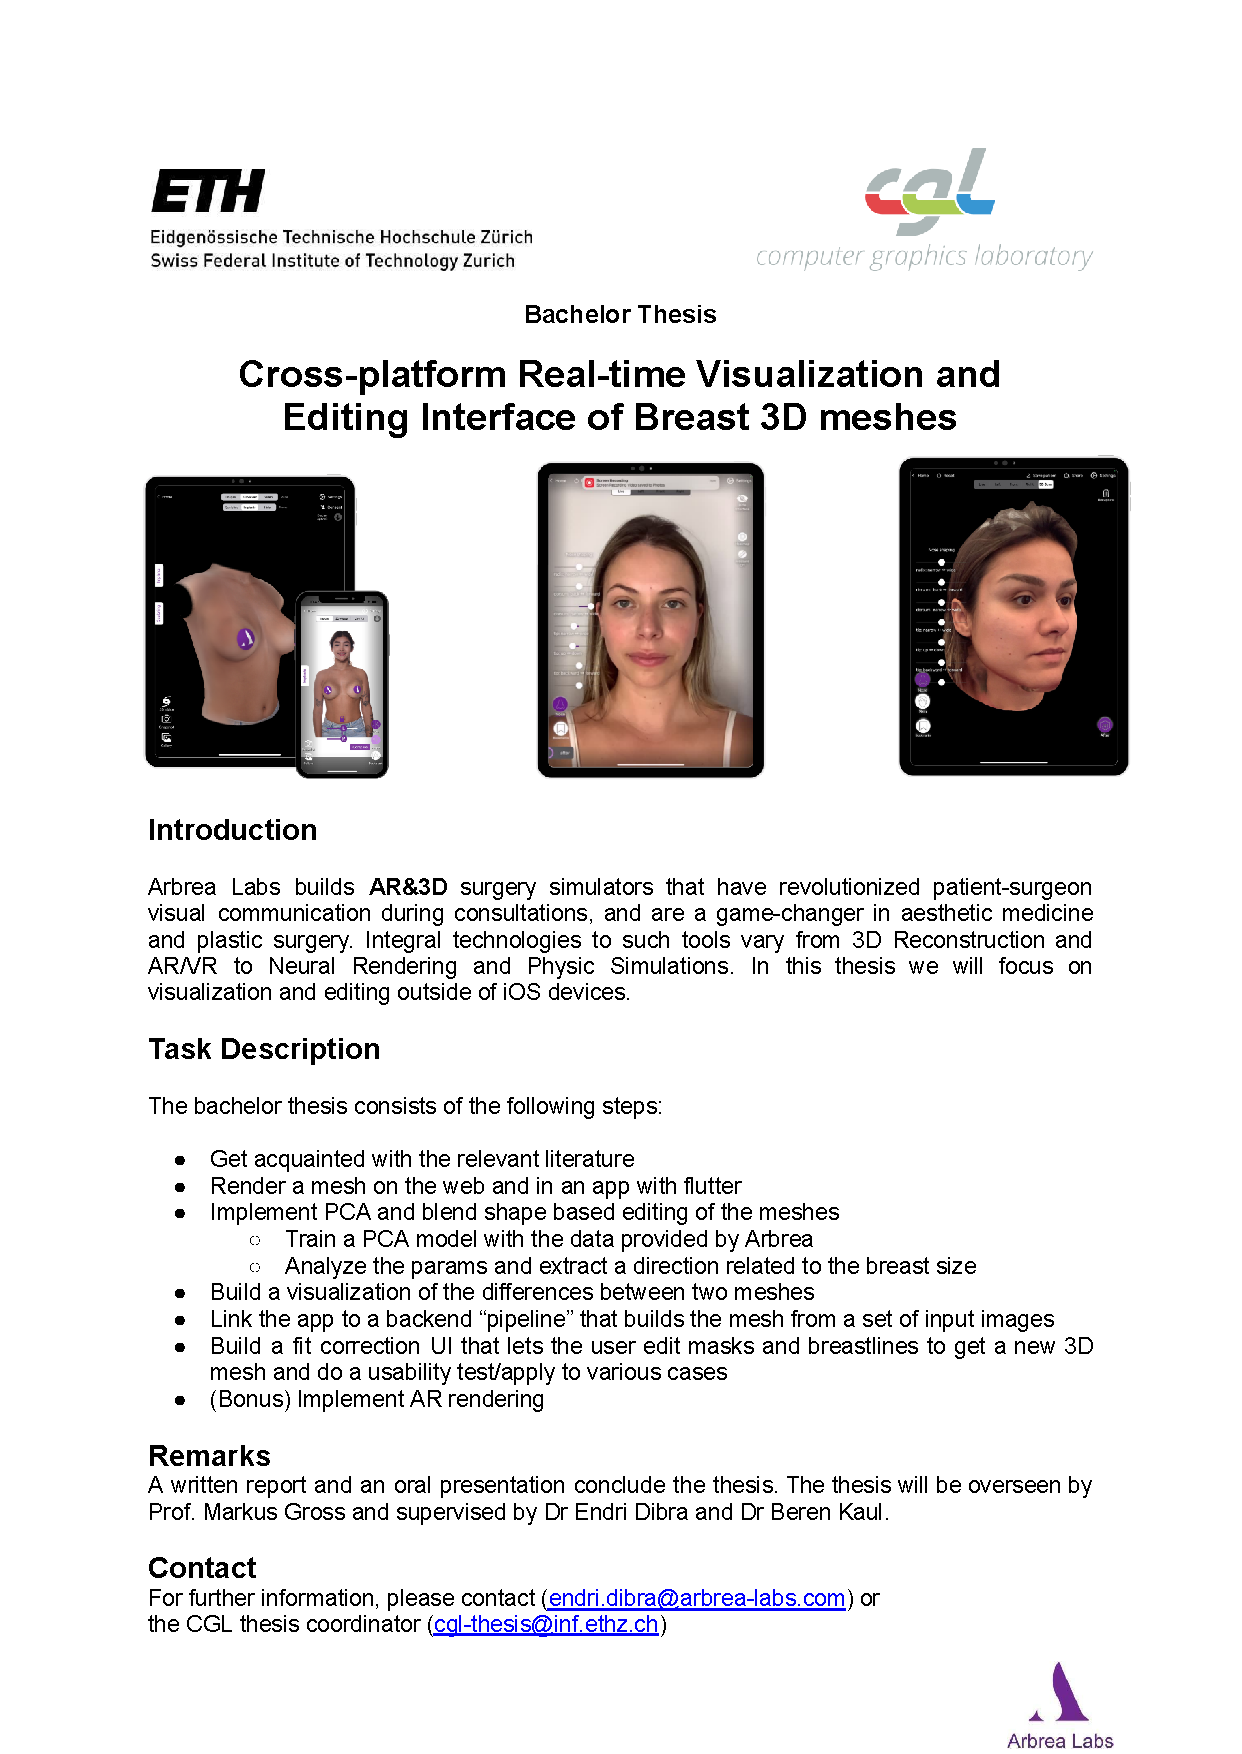
\includepdf[page={1}]{Luca_Sichi_Thesis_description}
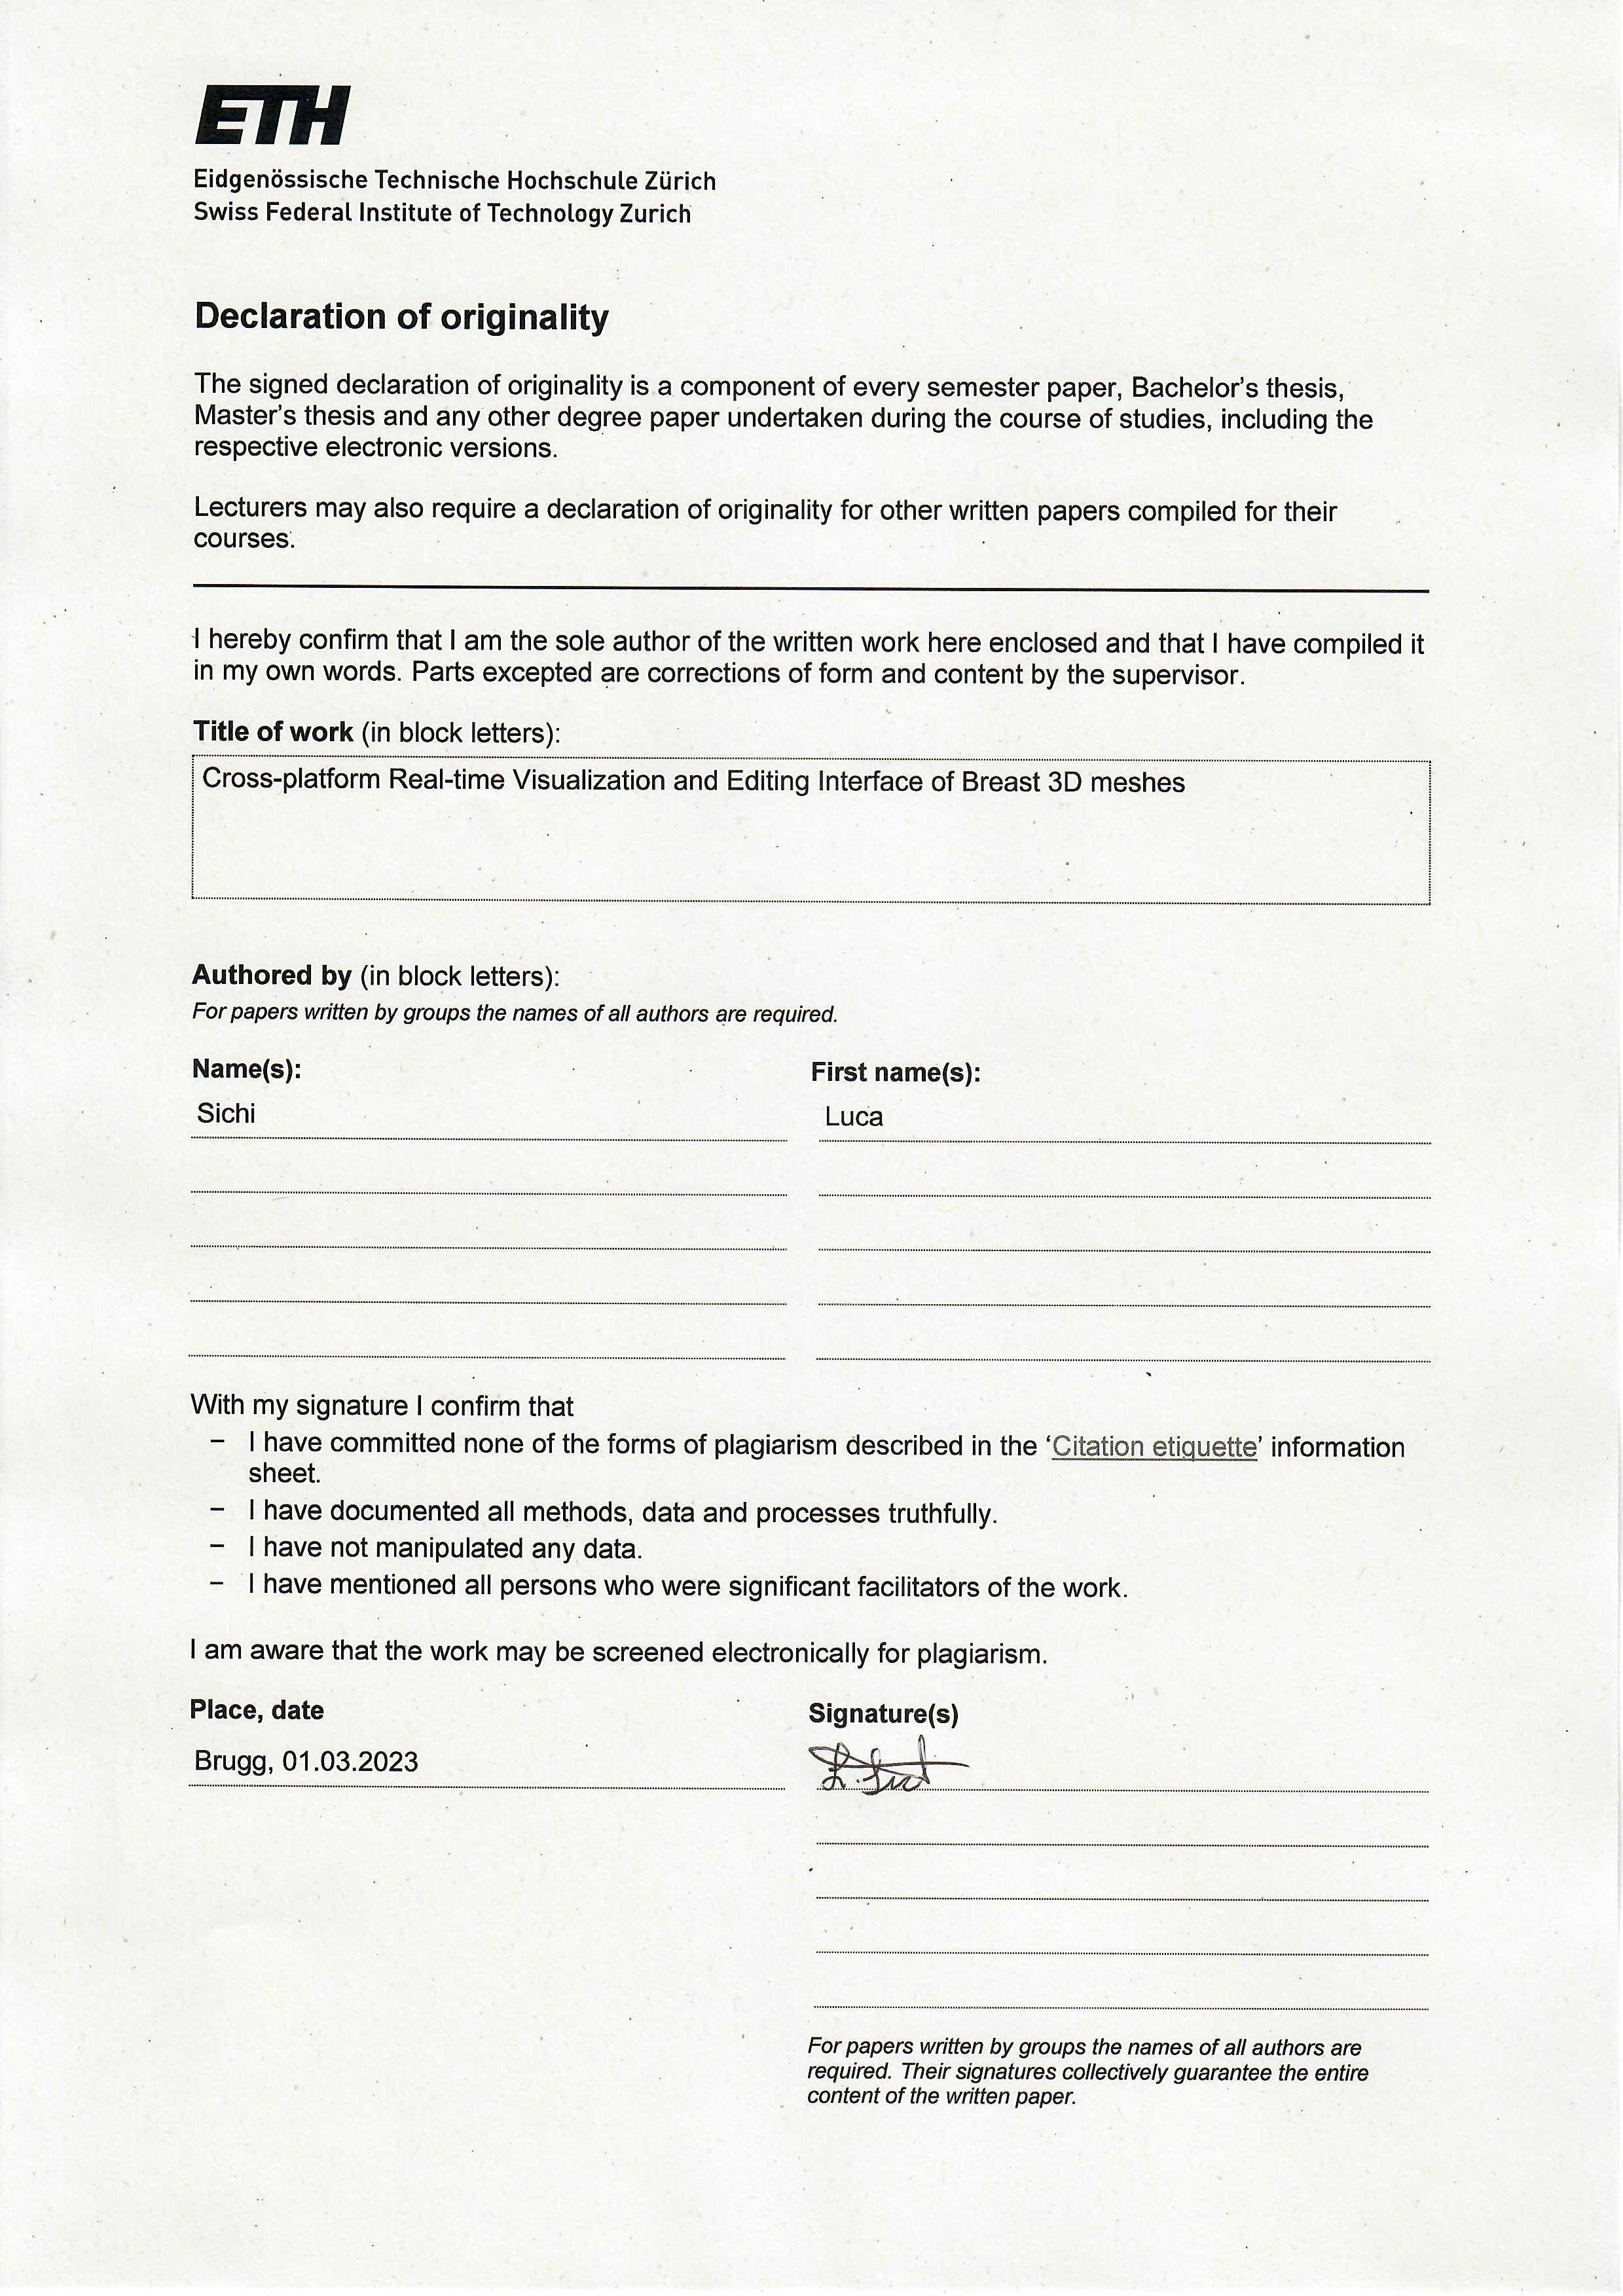
\includepdf[page={1}]{declaration_of_originality}

\includepdf[page={1}]{blank}

\includepdf[page={1}]{blank}

\includepdf[page={1}]{blank}
\end{document}
